\section{\"Ubertragungsverhalten}
In diesem Versuchsteil wird das \"Ubertragungsverhalten des Operationsverst\"arkers analysiert. 
\subsection{Experimentelle Durchf\"urung}
Es sollte der nicht invertierende Verst\"arker mit A$_{d_0}$ $=$ 5 wie in Abbildung 6 zu sehen ist, aufgebaut werden. Zun\"achst wird die Kennlinie der Ausgangsspannung U$_a$ als Funktion der Eingangspannung U$_e$ aufgenommen. Das Ergebnis soll mit der PSpice Simulation verglichen werden. Danach sollte der Betrag und die Phase bestimmt werden. F\"ur die Messung sollte ein logarithmischer Frequenzbereich gew\"alt werden. Im zweiten Versuchsteil wird die Verst\"arkung des nicht invertierenden Verst\"arkers auf A$_{d_0}$ $=$ 50 vergr\"o\ss ert, und es sollte wiederum der Betrags- und Phasengang bestimmt werden. Zum Schluss sollten die Betrags-und Phaseng\"ange der unterschiedlichen Verst\"arkung miteinander verglichen werden.
\subsection{Ergebnisse und Diskussion}
Man kann erkennen, dass der Operationsverst\"arker solange linear verst\"arkt bis er die Betriebspannung erreicht hat. Dieses Verhalten kann man sowohl in der Messung als auch in der Simulation erkennen(Abbildung 7 bzw. 8). Wobei der Theoretische Wert von der Betriebspannung bei der Messung nicht erreicht wird(bei ca. 11,4~$V$), da nicht mit idealen Bauteilen gearbeitet wird. 
\begin{figure}[!ht]
\begin{center}
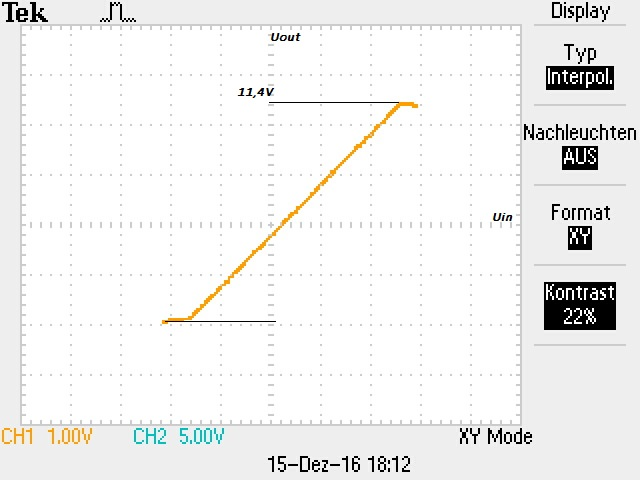
\includegraphics[scale=0.55]{bild/image4}
\caption{\"Ubertragungsverhalten des Operationsverst\"arker(Gruppe 14, Donnerstag)}
\end{center}
\end{figure}
\begin{figure}[!ht]
\begin{center}
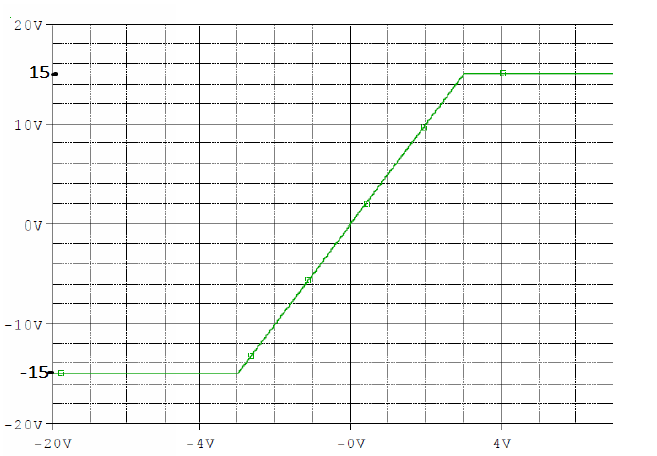
\includegraphics[scale=0.55]{bild/ubertragunsverhalten}
\caption{\"Ubertragungsverhalten des Operationsverst\"arker Simulation(U$_{\text{in}}$ x-Achse, U$_{\text{out}}$ y-Achse}
\end{center}
\end{figure}
\begin{figure}[!ht]
\begin{center}
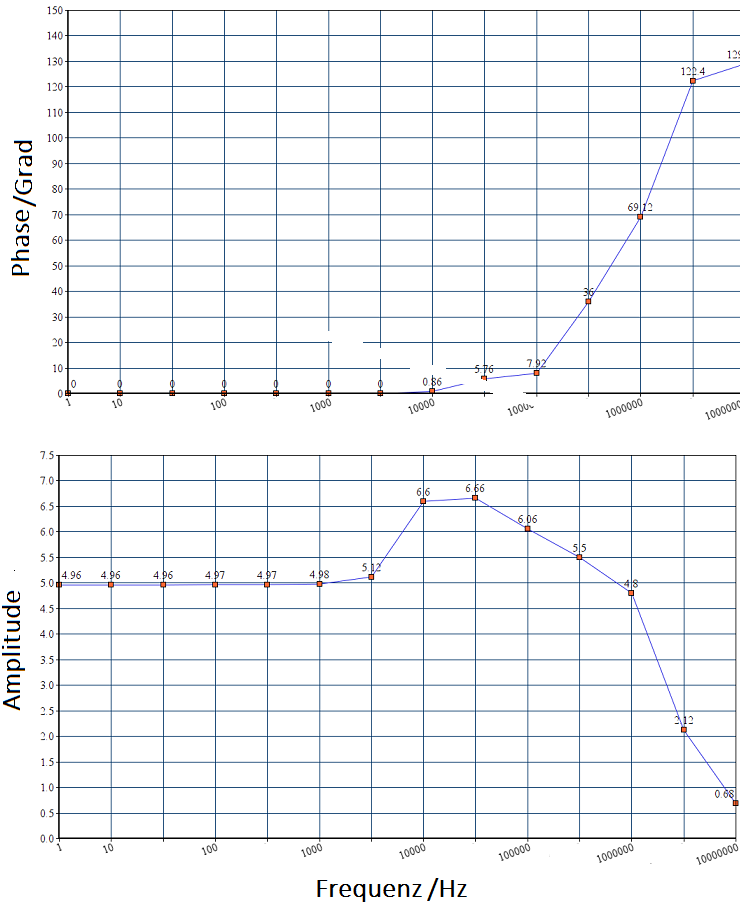
\includegraphics[scale=0.6]{bild/Phasengang5A}
\caption{Phasen- und Amplitudengang mit A=5}
\end{center}
\end{figure}
Aus unseren Messergebnisse ergaben sich folgende Schaubilder (Abbildung 9-15), jeweils f\"ur A$_{d0}$=5 und A$_{d0}$=50. Es Zeigt sich, dass eine Vergr\"o\ss erung der Verst\"arkung von 5 auf 50 kaum ein Einflu\ss auf die Schaubilder haben, die Ungenauigkeiten lassen sich durch Messfehler bzw. Messungenauigkeiten zur\"uck f\"uren.\\
\noindent
Zu erkennen ist, dass es sich beim Operationsverst\"arker um einen Tiefpass handelt, da dessen Verst\"arkungsverhalten bei gr\"o\ss ere Frequenzen absinkt. Dieses Verhalten ist aus Stabilit\"atsgr\"unden charakteristisch f\"ur einen Operationsverst\"arker